%Title:  What has been tried for system 8 and what is example.
 
\documentclass[11pt]{article}
\usepackage{amssymb,latexsym,amsmath}
\usepackage{graphicx}
\usepackage{epsfig}
\usepackage{enumerate}
\usepackage[top=1in,right=1in,left=1in,bottom=1in]{geometry}

%-----------------------------------------------------------------
\vfuzz2pt % Don't report over-full v-boxes if over-edge is small
\hfuzz2pt % Don't report over-full h-boxes if over-edge is small
% THEOREMS -------------------------------------------------------
%\theoremstyle{remark}
%\newtheorem*{rem}{Remark}
% MATH -----------------------------------------------------------
\newcommand{\abs}[1]{\left\vert#1\right\vert}
\newcommand{\set}[1]{\left\{#1\right\}}
\newcommand{\Real}{\mathbb R}
\newcommand{\Z}{\mathbb Z}
\newcommand{\Q}{\mathbb Q}
\newcommand{\To}{\rightarrow}
\newcommand{\display}[1]{\begin{displaystyle}#1\end{displaystyle}}
\renewcommand{\phi}{\varphi}
%\newtheorem{theorem}{Theorem}[section]
%\newtheorem{lemma}[theorem]{Lemma}
%\newtheorem{proposition}[theorem]{Proposition}
%\newtheorem{corollary}[theorem]{Corollary}

\newenvironment{proof}[1][Proof]{\begin{trivlist}
\item[\hskip \labelsep {\bfseries #1}]}{\end{trivlist}}


\newenvironment{definition}[2][Definition]{\begin{trivlist}
\item[\hskip \labelsep {\bfseries #1} \hskip .1em {\bfseries #2}]}{\end{trivlist}}
\newenvironment{theorem}[2][Theorem]{\begin{trivlist}
\item[\hskip \labelsep {\bfseries #1} \hskip .1em {\bfseries #2}]}{\end{trivlist}}
\newenvironment{proposition}[2][Proposition]{\begin{trivlist}
\item[\hskip \labelsep {\bfseries #1} \hskip .1em {\bfseries #2}]}{\end{trivlist}}
\newenvironment{lemma}[2][Lemma]{\begin{trivlist}
\item[\hskip \labelsep {\bfseries #1} \hskip .1em {\bfseries #2}]}{\end{trivlist}}
\newenvironment{corollary}[2][Corollary]{\begin{trivlist}
\item[\hskip \labelsep {\bfseries #1} \hskip .1em {\bfseries #2}]}{\end{trivlist}}
\newenvironment{note}[1][Note]{\begin{trivlist}
\item[\hskip \labelsep {\bfseries #1}:]}{\end{trivlist}}

\newenvironment{example}[1][Example]{\begin{trivlist}
\item[\hskip \labelsep {\bfseries #1}]}{\end{trivlist}}
\newenvironment{remark}[1][Remark]{\begin{trivlist}
\item[\hskip \labelsep {\bfseries #1}]}{\end{trivlist}}

\newcommand{\qed}{\nobreak \ifvmode \relax \else
      \ifdim\lastskip<1.5em \hskip-\lastskip
      \hskip1.5em plus0em minus0.5em \fi \nobreak
      \vrule height0.75em width0.5em depth0.25em\fi}
% ----------------------------------------------------------------
%\setlength{\topmargin}{-.3in}
%\setlength{\headheight}{.2in}
%\setlength{\headsep}{.3in}
%\setlength{\oddsidemargin}{0in}
%\setlength{\evensidemargin}{0in}
%\setlength{\textwidth}{6.5in}
%\setlength{\textheight}{8.5in}
\renewcommand{\baselinestretch}{1.2}
% ----------------------------------------------------------------
\pagestyle{empty}

\begin{document}

\begin{center}{\Large{\textbf{Report Outline}}}
\end{center}


\vspace{.2in}

\section{Abstract}

	\begin{enumerate}
		\item A mechanical switch involving a spring can have many uses. 
		
		\item Depending on the desired use of the spring, an optimal spring will be different. 
	
		\item To find an optimal spring we need to have a set of constraints and objectives to optimize. 
		
		\item The constraints and objectives are subject to change depending on the use. 
		
		\item The objective of this project is to design a flexible optimization routine, that is, flexible in what constraints and objectives are considered. 
		
	\end{enumerate}
	
\section{Introduction}
	\begin{enumerate}

		\item To be flexible in finding an optimum spring you must allow for constraints and objectives to be interchangeable.
				
		\item There also exists constraints and objectives that are informed by real-world tolerances for design and fabrication. 
	
		\item In order to allow this flexibility we employ the use of object oriented programming techniques. 
		
		\item In addition, we must be able to find an optimal spring that is subject to constraints, and tolerances that are set by 
		
		\item 
		
	\end{enumerate}
	
	\section{Helical Compression Springs}
	\begin{enumerate}
		\item Work done on the design given uncertainty in an acceleration switch, IMECE2011 paper.
		
	\end{enumerate}	
		

Helical springs are a large class of springs sharing the common characteristic of a coiled appearance (see figure).  Below is a list of a spring's key design parameters.

		\begin{enumerate}
			\item Spring's inner diameter $d_{i}$ 
			\item Spring's outter diameter $d_{o}$
			\item Spring's coil width $d_{w}$
			\item Total number of spring coils $N_{t}$
			\item Pitch $p$
			\item Spring's free length $L_{free}$
			\item Spring's solid length $L_{solid}$
			\item Spring's open length $L_{open}$
			\item Spring's shear modulus $G$
		\end{enumerate}

These various characteristics interact to define key attributes of the spring.

	\begin{enumerate}
		\item \textbf{Spring Rate} - this is the effective stiffness of the spring in compression.
\begin{align*}
		k = \dfrac{G}{8 N_{a} (ec)} \dfrac{d_{w}^{4}}{(d_{i}+d_{w})^{3}}
\end{align*}
		\item \textbf{Spring Index} - indicates the distribution and magnitude of stress.
\begin{align*}
		C = \dfrac{d_{i}}{d_{w}} + 1
\end{align*}
		\item Coil Binding Gap
\begin{align*}
	g = \dfrac{L_{hard} - L_{solid}(d_{w},N_{a}; ec)}{N_{t} - 1}
\end{align*}
		\item Maximum Shear Stress
\begin{align*}
		\dfrac{G(L_{free} - L_{hard})}{4 \pi N_{a} (ec)} [\dfrac{d_{w} (4d_{i}^{2} + 9.46d_{i} 
d_{w} + 3 d_{w}^{2})}{d_{i}(d_{i}+d_{w})^{3}}] < UTS
\end{align*}
	\end{enumerate}


\section{Problem Formulation}

	\begin{enumerate}
	
		\item The formulation is informed by many sources... 
				
		\item Multiple-Interconnected Dimensions, graph of interconnectedness
	
		\item List the properties and a short description.

		

		\item Illustrate example of optimization, and explain our generalization.
		
		\item Relaxation and Creep
		
	\end{enumerate}
	
	
\section{Approach to Problem}

\subsection{Software Design}
	\begin{enumerate}
	
		
		
		\item Flexibility integrated into existing optimization.
				
		\item Constraint vs. Objective
	
		\item A constraint is an expression that must satisfy an inequality or equality condition.
		
		\item An objective is an expression that can be evaluated.
		
		\item So an constraint can be an objective. 
		
	\end{enumerate}
	
\section{Workflow}
	 \begin{center}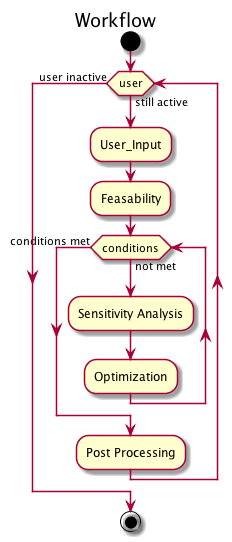
\includegraphics[scale=.5]{IMSM_Workflow.png}\end{center}

\subsection{Feasibility}
	\begin{enumerate}
		\item 
	\end{enumerate}

\subsection{Sensitivity Analysis}
\hspace{5 mm} As the dimension of design variable space increases, the computational expense of the optimization procedure increases. To reduce the computational expense, it is often desirable to reduce the design variable space by removing the variables that have very little influence on the objective function. Thus, a dimension reduction strategy is required to reduce the design variable space. Dimension reduction approaches, in the literature have been divided into two categories - (1)filter approach, and (2)wrapper approach. In the filter approach, the input variables are ranked according to a ranking criterion and the most dominant variables can be selected by assuming a threshold influence value. In the wrapper approach, a subset of variables is selected from the list of all possible subsets of the input variables that best estimate the output variable. An optimization technique is used to obtain the best subset of input variables. In this work, the variance-based Global Sensitivity Analysis (GSA), a filter approach, is used for dimension reduction. Note that the input variables represent the design variables for the objective function.

\hspace{5 mm} Consider a objective function, $G$, with $n$ design variables given by $x_{1}$, $x_{2}$, ...  $x_{n}$, given by

\centerline{$Y = G(x_{1}, x_{2}, ... x_{n})$}

In GSA, two types of indices can be calculated for each variable - first order index and total effects index. The first-order index ($S_{i}^{I}$) quantifies the uncertainty contribution of an input variable, without considering its interactions with other variables, to the output variable uncertainty. Similarly, the total effects index ($S_{i}^{T}$) quantifies the uncertainty contribution of an input variable by considering its interactions with all variables, to the output uncertainty. The expressions for the two sensitivity indices are given below as 

\centerline{$S_{i}^{I} = \dfrac{V_{X_i}(E_{X_{-i}}(Y|X_{i}))}{V(Y)}$}
\centerline{$S_{i}^{T} = \dfrac{E_{X_{-i}}(V_{X_{i}}(Y|X_{-i}))}{V(Y)}$}

Given a design range (lower and upper bounds), a variable can be assumed to be uniformly distributed in the design range. For each variable, the total-effects index is calculated and if it is less than an assumed threshold value, then that variable is assumed insensitive and removed from the optimization procedure. Thus, dimension reduction is implemented for a faster design optimization. 


\subsection{Optimization}
	\begin{enumerate}
		\item
	\end{enumerate}

		
\section{Computational Experiments}
	\begin{enumerate}

		\item Case Studies
		
		\item Relaxation and Creep
		
	\end{enumerate}
	
	
		
\section{Summary and Future Work}
	\begin{enumerate}
	
		
		
		\item Computational Inefficiencies 
				
		\item 
		
		\item 
		
		\item 
		
		\item 
		
	\end{enumerate}
	
	\section{References}
		

	\end{document}
